\documentclass[a4paper,10pt]{article}
\usepackage[utf8x]{inputenc}
\usepackage[spanish]{babel}
\usepackage{amsmath}
\usepackage{graphicx}
\usepackage{fullpage}

\newif\ifpdf
\ifx\pdfoutput\undefined
   \pdffalse
\else
   \pdfoutput=1
   \pdftrue
\fi
\ifpdf
   \usepackage{graphicx}
   \usepackage{epstopdf}
   \DeclareGraphicsRule{.eps}{pdf}{.pdf}{`epstopdf #1}
   \pdfcompresslevel=9
\else
   \usepackage{graphicx}
\fi

%opening
\title{Tutoría 4 - Estructuras de datos y algoritmos}
\author{Cristóbal Ganter y Felipe Vera}

\begin{document}

\maketitle

\paragraph{¡Aviso!} ¡Recuerde dejar la máquina virtual en orden una vez que termine su trabajo!
¡Pregunte al ayudante apenas tenga una duda!

Si tiene problemas de \textit{segmentation fault} o \textit{stack overflow} en su programa, una buena opción es \textit{debuggear} su programa con el comando \texttt{ddd nombre-de-programa}.
Estos errores son difíciles de encontrar, por lo que llenar su programa de \texttt{printf}s no lo ayudará mucho.

\paragraph{Contenido de esta semana}
\begin{itemize}
  \item punteros, punteros dobles y operador \&
  \item Asignación dinámica de memoria: stack, heap, \texttt{malloc} y \texttt{free}.
  \item Estructuras de datos dinámicas: árboles binarios y operaciones con ellos: búsqueda e inserción.
  \item Empleo de funciones recursivas para los contenidos anteriores.
\end{itemize}

\paragraph{Actividad}
\begin{enumerate}
 \item \textbf{Uso de los árboles binarios}

  Se usarán árboles binarios para modelar un \textit{parser aritmético}, es decir, una función que acepta un \textit{string} con una operación aritmética
  y regresa el resultado de tal operación.
  \begin{enumerate}
    \item Cree la estructura básica de un árbol binario. Defina un \texttt{struct \_parser} con los miembros \texttt{char operacion}, \texttt{double operando},
    \texttt{struct \_parser *leftchild} y \texttt{struct \_parser *rightchild}. Ocupe posteriormente \texttt{typedef} para referirse a esta estructura como
    un tipo \texttt{parser}.
    \item Escriba una función para crear un nodo, llamada \texttt{parser crear\_nodo}, que acepte como argumentos nuevos valores para \texttt{operacion} y
	  \texttt{operando}.
  \end{enumerate}

  \item \textbf{Crear el árbol a partir de una expresión sencilla: inserción}

  La función que usted creará ahora se limitará a operaciones de suma y resta, sin paréntesis y sin números negativos.

  \begin{enumerate}
    \item Cree una función \texttt{parser *crear\_arbol}, que acepte como argumento la cadena de caracteres. Ayúdese de la referencia de la librería de C para
	  dividir la cadena en operadores y números empleando \texttt{strtok}; y convertir los números a tipo \texttt{double} empleando \texttt{atof}.
    \item Tal función necesitará hacer una inserción simple en un árbol binario. Cree una función \texttt{void insertar\_numero (parser **top, double numero)} que inserte
	  un número como nodo hijo izquierdo. De existir el nodo hijo izquierdo, intenta al derecho.
    \item También se necesitará una inserción reemplazando el padre por el hijo izquierdo. Cree una función \texttt{void insertar\_operacion (parser **top, double numero, char op)}
	  que cambie al nodo apuntado por \texttt{*top} (un número) por la operación indicada, y lo baje al nodo hijo izquierdo. Como nodo hijo derecho, coloca
	  al nuevo número ofrecido como argumento a esta función.
    \item Implemente con estas dos nuevas funciones, haciendo crecer el árbol por la derecha. Pruebe la función de la manera que usted quiera: puede ser ingresando
	  datos por consola o en el mismo código.
  \end{enumerate}


  \item \textbf{Función para evaluar el árbol}

  El parser funcionará aceptando en el miembro \texttt{operacion} a los operandos \texttt{+}, \texttt{-}, \texttt{*}, \texttt{/}, \texttt{\^}, paréntesis y
  \texttt{n}. El último indicará que el miembro es una constante numérica, y en ese caso será cuando \texttt{operando} entre en acción.

  \begin{enumerate}
      \item Cree una función recursiva \texttt{double evaluar} que acepte como argumento el árbol \textit{parser} y devuelva el resultado de la
	    operación. Guíese por sus apuntes y siga un esquema como el siguiente. El siguiente árbol muestra, por ejemplo, el parser que devolvería
	    un árbol que fue creado con la operación \texttt{$10 * (0 - 12) + 60 + 35$}
      
      \centering
      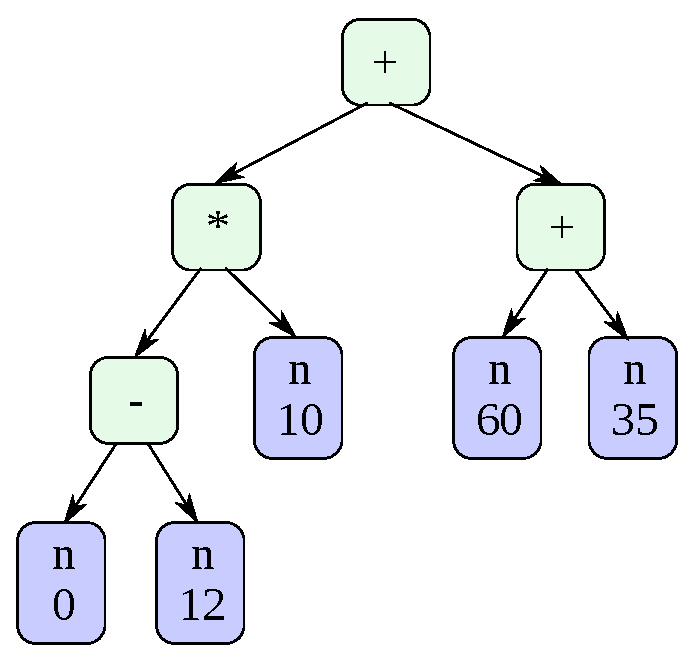
\includegraphics[scale=0.3]{esq_arbol.eps}

      
%     \item Cree una función \texttt{parser analizar\_string} que acepte como argumento un arreglo de \texttt{char} que contenga una expresión aritmética.
% 	  Oriéntese con lo que el ayudante explique en la pizarra.
%     \item Del mismo modo, cree una función recursiva \texttt{int evaluar} que acepte como argumento el árbol \textit{parser} y devuelva el resultado de la
% 	  operación.
%     \item Suponga que escribe bien la operación y ponga a prueba las funciones. Elabore un programa al cual se le ingresa la operación por consola y 
% 	  devuelva el resultado.
  \end{enumerate}

  \item \textbf{Prioridad de operaciones}

  Las potencias se hacen primero, luego las multiplicaciones y divisiones y por último las sumas y restas. Por ahora no ocuparemos los paréntesis.
  
  \begin{enumerate}
    \item Asigne un número de prioridad a cada operación: sumas y restas corresponden a 1, multiplicaciones y divisiones corresponden a 2, y potencias a 3.
	  Con ello, modifique las funciones \texttt{insertar\_operacion} y \texttt{crear\_arbol} para que se adecúen a la prioridad de las operaciones.
	  Se sugiere que \texttt{insertar\_operacion} sea recursiva.
  \end{enumerate}
  
  \item \textbf{Inclusión de paréntesis}

  Los paréntesis sirven para cambiar la prioridad de las operaciones.

  \begin{enumerate}
    \item Por cada signo de ``abrir paréntesis'', se suma 3 a la prioridad de la operación. Por ejemplo, una suma dentro de un paréntesis tendrá prioridad 4,
	  la multiplicación 5; y si están dentro de un paréntesis anidado, prioridad 7 y 8 respectivamente. Haga los cambios respectivos a las funciones necesarias
	  para que respeten los paréntesis.
    \item Por último, pruebe el código ingresando una expresión por consola como argumento. 
  \end{enumerate}

\end{enumerate}

\end{document}
